% !TeX document-id = {ac384373-0975-4c4e-b6b2-65611dc82067}
% !TeX TXS-program:compile = txs:///pdflatex/[--shell-escape]
\documentclass[a4paper,12pt]{article}

\usepackage[T2A]{fontenc}
\usepackage[russian]{babel}
\usepackage[intlimits,namelimits]{amsmath}
\usepackage{amssymb}
\usepackage{mathtools}
\usepackage{mathrsfs}
\usepackage{geometry}
\usepackage[color={1 0 .5}]{attachfile2}

\usepackage{indentfirst}
\usepackage{icomma}
\usepackage{graphicx}
\usepackage{geometry}
\usepackage{setspace}
\usepackage{fancyhdr}
\usepackage{titlesec}
\usepackage{minted}
\usepackage{float}
\usepackage{caption}
\usepackage{rotating}

\usepackage{minted}

%%\usepackage[bibstyle=gost-numeric,citestyle=numeric-comp]{biblatex}

\usepackage{hyperref}

%%\addbibresource{biblio.bib}

\geometry{a4paper, nomarginpar, left=20mm, right=10mm, top=20mm, bottom=20mm}

\setlocalecaption{russian}{ref}{Список литературы}


\newcommand\Vect[1]{{\boldsymbol{#1}}}
\newcommand{\dd}{\mathrm{d}}
\newcommand{\diag}{\operatorname{diag}}
\renewcommand{\Re}{\operatorname{Re}}
\renewcommand{\Im}{\operatorname{Im}}
\renewcommand{\exp}{\operatorname{e}}
\renewcommand{\imath}{\mathrm{i}}
\newcommand{\trp}{\mathrm{T}}

\newcommand{\mintedlabel}[1]{\phantomsection\label{\detokenize{#1}}}


% \DeclarePairedDelimeter\bra{\langle}{|}
\DeclarePairedDelimiter\ket{|}{\rangle}
\DeclarePairedDelimiter\abs{\lvert}{\rvert}
\DeclarePairedDelimiterX\commut[2]{[}{]}{#1,#2}
\DeclareCaptionLabelFormat{figRu}{Рисунок~#2}
\DeclareCaptionLabelSeparator{figRuSep}{~---~}
\captionsetup[figure]{labelformat=figRu,labelsep=figRuSep}

%\titleformat{\subsection}[block]{\filcenter}{\thesubsection}{0.5em}{}
\titleformat{\section}{\normalfont\Large\bfseries}{\thesection.}{1em}{}
\titlespacing{\section}{\parindent}{3.5ex plus 1ex minus .2ex}{2.3ex plus .2ex}
\titlespacing{\subsection}{\parindent}{3.5ex plus 1ex minus .2ex}{2.3ex plus .2ex}
\titlespacing{\subsubsection}{\parindent}{3.5ex plus 1ex minus .2ex}{2.3ex plus .2ex}

\fancypagestyle{plain}{%
	\fancyhf{}%
	\fancyfoot[R]{\thepage}%
	\renewcommand{\headrulewidth}{0pt}%
	\renewcommand{\footrulewidth}{0pt}%
}

%%%%%%%%%%%%%%%%%%%%%%%%%%%%%%%%%%%%%%%%%%%%%%%%%%%%%%%%%%%%%%%%%%%%%%%%%%%%%%%%

\makeatletter
\def\@sect[#1]#2{%
	\refstepcounter{app@section}
	\setcounter{equation}{0}
	\addcontentsline{toc}{section}{Приложение~\theapp@section}
	{%
		{
			\raggedleft%
			\normalfont%
			Приложение~\theapp@section\par%
		}%
		\Large\bfseries%
		#2%
		\par%
	}
	\vskip 3ex
}
% This is supposed to be "starred" version, but it doesn't have sense in the
% appendix, so we simply repeat above definition.
\def\@ssect#1{%
	\refstepcounter{app@section}
	\addcontentsline{toc}{section}{Приложение~\theapp@section}%
	{%
		{%
			\raggedleft%
			\normalfont%
			Приложение~\theapp@section\par%
		}%
		\Large\bfseries%
		#1%
		\par%
	}%
	\vskip 3ex
}

\renewcommand\appendix{%
	\newpage%
	\newcounter{app@section}
	\setcounter{app@section}{0}
	%\setcounter{equation}{0}%
	\renewcommand\theapp@section{\Asbuk{app@section}}
	\renewcommand\theequation{\theapp@section\arabic{equation}}
	%%% We need to redefine \section command here...
	%%% NB: this is messy, VERY messy (see GOST for autoreferat!)
	\renewcommand{\section}{%
		\secdef\@sect\@ssect
	}
}

%%%%%%%%%%%%%%%%%%%%%%%%%%%%%%%%%%%%%%%%%%%%%%%%%%%%%%%%%%%%%%%%%%%%%%%%%%%%%%%%

\allowdisplaybreaks[4]
\begin{document}

\onehalfspacing
\pagestyle{plain}

\begin{titlepage}
	\begin{center}%
		Министерство науки и высшего образования Российской Федерации\\
		Федеральное государственное бюджетное образовательное учреждение\\
		высшего образования \\
		«Иркутский государственный университет»\\
		(ФГБОУ ВО «ИГУ»)\\
	\end{center}
	\vspace*{3em}
	
	\begin{flushright}
		\begin{minipage}{92mm}
			Физический факультет\\
			Кафедра теоретической физики\\
			Зав. кафедрой Доцент, к.ф.-м.н.\\
			Ловцов С.В. \underline{\hspace{35mm}}
		\end{minipage}
	\end{flushright}
	\vspace*{4em}
	
	\begin{center}
		\Large
		\bfseries%
		ОТЧЕТ ПО ПРОИЗВОДСТВЕННОЙ ПРАКТИКЕ\\
		«Преддипломная практика»\\[2ex]
		Расчёт качественной характеристики уравнения осцилляций нейтрино в среде по методу Магнуса
	\end{center}
	
	\vspace*{3em}
	
	\begin{flushright}
		\begin{minipage}{95mm}
			Руководитель практики: \underline{\hspace{35mm}}\\
			Ломов В.П., к.ф.-м.н., доцент\\[2ex]
			Студент гр. 01411-ДБ\\
			\underline{\hspace{35mm}}/Данеко Илья Игоревич\\[2ex]
			Работа защищена с оценкой \underline{\hspace{30mm}}\\
			<<\underline{\hspace{8mm}}>>\underline{\hspace{22mm}}2026г.\\
			Нормконтролёр\\
			\underline{\hspace{35mm}}/Фролова А.С./\\
		\end{minipage}
	\end{flushright}
	
	\vfill
	\begin{center}
		Иркутск 2026
	\end{center}
\end{titlepage}

\setcounter{page}{2}

\thispagestyle{empty}
\tableofcontents

\newpage

	\section*{Введение}
	\addcontentsline{toc}{section}{Введение}
Нейтринная физика сейчас является одним из рубежей современной физики. Также благодаря своим необычным свойствам нейтрино являются важным элементом для построения моделей за пределами стандартной модели.

Нейтрино --- это общее название нейтральных фундаментальных частиц с полуцелым спином, участвующих только в слабом и гравитационном взаимодействиях, и относящихся к классу лептонов. Наиболее важным открытием в физике нейтрино стало наблюдение осцилляций, которые к настоящему моменту подтверждены многочисленными экспериментами с солнечными, атмосферными, реакторными и ускорительными нейтрино.

Идея нейтринных осцилляций была предложена Бруно Понтекорво в 1957-1958 годах, она была основана по аналогии с K-мезонами \cite{11, 22}. Уже в 1962 году, Маки, Накагавой и Сакатой была разработана теория смешивания нейтрино в вакууме \cite{33}. В 1963 году Накагавой, Окониги, Сакатой и Тойодой была предложена связь между перемешиванием нейтрино с определенным флейвором и нейтрино с определённой массой \cite{44}. Вольфенштейном было обращено внимание на эффект при распространении нейтрино через обычное вещество (среда электронейтральная, немагнитная, нерелятивистская) в 1978 году \cite{55, 66}. В 1986 году Михеевым и Смирновым этот эффект был физически описан (MSW-эффект) \cite{77, 88}. И наконец, в 2015 году в качестве доказательства осцилляций нейтрино были признаны результаты SNO (Садберийская нейтринная обсерватория) \cite{99} и Super-Kamiokande \cite{1010}.

По сравнению с вакуумными осцилляциями нейтрино, при изучении осцилляции нейтрино в веществе, все сложнее. Поэтому в таком случае, как правило, применяют численные расчёты.

Основной целью данной работы стоит поиск качественной характеристики численного решения уравнения осцилляции нейтрино в среде.

В первом разделе мы приводим краткие сведения по альтернативному методу интегрирования уравнения шрёдингеровского типа. Получаем данные численного решения уравнения осцилляций в среде с помощью данного метода.

Во втором разделе мы кратко рассматриваем конкретный метод, что будет использоваться.

В третьем разделе мы получаем данные численного решения уравнения осцилляций в среде с помощью данного метода.

	\newpage
\section{Геометрический интегратор}

		Нам нужно решить уравнение осциляции нейтрино в среде
	\begin{equation}\label{eq:15}
		\imath\frac{\dd\Psi(\xi)}{\dd\xi}=[H_{0}+ v(\xi)W]\Psi(\xi),
	\end{equation}
	с начальным условием
	\begin{equation}\label{eq:19}
		\Psi(\xi_0)=
		\begin{pmatrix}
			c_{13}c_{12}\\
			s_{12}c_{13}\\
			s_{13}
		\end{pmatrix}.
	\end{equation}
	Его особенности: матричное уравнение, матрица в правой части не коммутирует сама в собой в разных точках и самое важное — она эрмитова.

Для его решения рассмотрим более общую задачу. Пусть дана матрица \(A(t)\) \(n\times n\) и уравнение вида
	\begin{equation}\label{eq:41}
		\frac{\dd y(t)}{\dd t}=A(t)y(t),\qquad y(t_0)=y_0,\qquad A\in C^{n \times n},\qquad y\in C^{n}.
	\end{equation}

Для решения уравнения \eqref{eq:41} воспользуемся подходом, описанным в \cite{Casas:2016asi, shay, ped}. Он называется методом Магнуса. Суть метода заключается в представлении искомой функции в виде
	\begin{equation}\label{eq:42}
		y(t)=\exp^{\Omega(t,t_0)}y_0,
	\end{equation}
 	причём
	\begin{equation}\label{eq:48}
		\Omega(t,t_0)\in C^{n \times n},\qquad \Omega(t_0,t_0)=0.
	\end{equation}
	Когда матричные элементы \(A\) являются независимыми от \(t\), тогда \(\Omega(t,t_0)=(t-t_0)A\). В общем случае \(\Omega(t,t_0)\) задаётся в виде разложения в ряд
	\begin{equation}\label{eq:44}
		\Omega(t,t_0)=\sum_{k=1}^{\infty}\Omega_{k}(t,t_0),\qquad \Omega(t_0,t_0)=0
	\end{equation}
	где слагаемое \(\Omega_{k}\) состоит из кратных интегралов от вложенных коммутаторов k матриц A, вычисленных в k разных моментов времени. Сложность отдельных слагаемых в значительной степени возрастает с увеличением индекса k. В частности, первые три из них считаются следующим образом
	\begin{equation}\label{eq:47}
		\begin{lgathered}
			\Omega_{1}=\int_{t_0}^{t}\dd t_1 A_1,\\
			\Omega_{2}=\frac{1}{2}\int_{t_0}^{t}\dd t_1 \int_{t_0}^{t_1}\dd t_2[ A_1,A_2],\\
			\Omega_{3}=\frac{1}{6}\int_{t_0}^{t}\dd t_1 \int_{t_0}^{t_1}\dd t_2 \int_{t_0}^{t_2}\dd t_3([[ A_1,A_2],A_3]+[A_1,[ A_2,A_3]]),\\
		\end{lgathered}
	\end{equation}
	здесь \(A(t_i)=A_i\), а квадратные скобки обозначают коммутатор: \([A,B]=AB-BA\).

	Согласно формулам \eqref{eq:42}, \eqref{eq:47} нам нужно вычислять интегралы. Они при численных вычислениях, тоже считаются числено. Для этого мы можем взять множество из узлов сетки \(t_1,t_2,...,t_N\), для которых \(n\)-ый шаг: \(h_n=t_{n+1}-t_n\), где \(0<n<N-1\).

	Далее определим что
	\begin{equation}\label{eq:45}
		y(t_{n+1})=\exp^{\Omega(t_n+h_n,t_n)}y(t_n).
	\end{equation}
	После этого благодаря  итерации мы можем записать решение в N шагов
	\begin{equation}\label{eq:43}
		y(t_{n+1})=\prod_{n=0}^{N-1} \exp^{\Omega(t_n;h_n)}y_0,\qquad \Omega(t_n;h_n)=\Omega(t_n+h_n,t_n).
	\end{equation}

	Для применения такого метода ряд \eqref{eq:44} нужно усечь
	\begin{equation}\label{eq:46}
		\Omega^{(p)}(t,t_0)=\sum_{k=1}^{p}\Omega_{k}(t,t_0),
	\end{equation}
	чтобы понять после какого члена усекать, необходимо узнать порядок аппроксимации метода. Он определяется, как порядок \(r\)-го разложения Тейлора, которое даёт \(y(t_{n}+h_n)\) вплоть до \(O(h_n^{r+1})\) из точного значения \(y(t_{n})\). Поскольку порядок квадратур, необходимый для численной аппроксимации \(\Omega_{k}\) в усечённый ряд не превышает порядка аппроксимации \(r\). А та как метод Магнуса симметричен по времени, для достижения метода интегрирования порядка \(2r\) (при \( r > 1\)) в разложении в ряд \eqref{eq:44} требуются только члены до \(p = 2r - 2\).

	Система дифференциальных уравнений, управляющая эволюцией амплитуд трёх нейтрино в веществе \eqref{eq:15}, она подходит под тип уравнений, описанный в \eqref{eq:41}, при \(n=3\), \(t=\xi\) и
	\begin{equation}
		A=-iH,\qquad y=\Psi,
	\end{equation}
	где \(H=H_{0}+ v(\xi)W\).

	Теперь мы применим подход, описанный выше, для численного решения такого уравнения с начальным условием \eqref{eq:19}. Из \eqref{eq:45} получим
	\begin{equation}
		\Psi(\xi_{n+1})=\exp^{\Omega^{[r]}(\xi_n;h_n)}\Psi(\xi_n),
	\end{equation}
	где \(\Omega^{[r]}\) обозначает приближение к усечённому ряду Магнуса \eqref{eq:46} порядка \(r\) по \(h_n\)

\newpage
\section{Метод M4}

	При \(p = 2\) в усечённом ряду \eqref{eq:46}, мы получаем метод порядка \(r = 4\). Если соответствующие интегралы \(\Omega_{1}\) и \(\Omega_{2}\) из \eqref{eq:47} аппроксимируются двухточечным правилом Гаусса-Лежандра \cite{68}. В частности, учитывая Квадратурные точки (узлы)
	\begin{equation}
		\xi_{\pm} = \xi_{n} + (1 \pm \frac{1}{\sqrt{3}})\frac{h_n}{2},
	\end{equation}
	где \(\xi_{-}<\xi_{+}\) и
	\begin{equation}
		H_{\pm} = H(\xi_{\pm}),
	\end{equation}
	одноступенчатый показатель интегрирования порядка 4 может быть приведён к виду
	\begin{equation}\label{eq:49}
		\Omega^{[4]}(\xi_n;h_n)=-i(H_+ + H_-)\frac{h_n}{2} +
\frac{\sqrt{3}}{12}[H_-, H_+]h_n^2.
	\end{equation}
	Здесь, как и прежде, квадратные скобки обозначают коммутатор.

	Вычисляя уравнение \eqref{eq:49} раскрыв матрицу H,  мы приходим к
	\begin{equation}
		\Omega^{[4]}(\xi_n;h_n)=-i(H_0 + \frac{1}{2}(\nu_+ + \nu_-)W)h_n +
\frac{\sqrt{3}}{12}(\nu_+ - \nu_-)[H_0, W]h_n^2,
	\end{equation}
	где \(\nu_{\pm} \equiv \nu(\xi_{\pm})\) --- единственные величины, которые необходимо повторно вычислять на каждом шаге интегрирования. Матрица \([H_0,W]\) создаётся только один раз в начале процесса интегрирования.

\newpage
\section{Обработка данных с метода M4}

	Перед нами всё также стоит задача найти качественные характеристики численного решения уравнения осцилляции нейтрино в среде. Так как данные полученные с помощью Дормана--Принса в \textsf{Wolfram Mathematica} имели выбросы было принято решение сделать такие же расчёты с помощью метода M4 вместо Дормана--Принса. Также мы использовали вместо \textsf{Wolfram Mathematica} код на \textsf{Python} для алгоритма и \texttt{magexp} программа, для численного решения при помощи метода Магнуса, а именно M4.

Мы поставили задачу найти качественные характеристики численного решения уравнения осцилляции нейтрино в среде. Из численного анализа мы заметили, что реальная и мнимая часть \(\psi_1\) часто пересекают ось абсцисс, однако к правой границе области они выходит на асимптотическое поведение, более не пересекая ось абсцисс. Из подобных соображений было принято решение узнать как распределены нули \(\psi_{1}\). Для этого было введено понятие квазипериода. Квазипериод --- это длина отрезка содержащего в себе 3 точки в которых функция  (в нашем случае реальная или мнимая часть \(\psi_1\)) зануляется, причём 2 из них являются границами этого отрезка.

Мы можем считать квазипериод функцией от точки \(\xi_0\) интервала \([0,1 ; 1]\) в таком смысле: находим 3 ближайших к \(\xi_0\) значения \(\xi\) при которых функция зависящая от \(\xi\) (в нашем случае реальная или мнимая часть \(\psi_1(\xi)\)) зануляется. Расстояние между крайними из них и есть искомый квазипериод в точке \(\xi_0\).

Нас заинтересовало поведение квазипериода на всём интервале \([0,1 ; 1]\). Вполне логично построить график зависимости квазипериода от \(\xi\). Для получения данных по всему интервалу мы воспользовались тем, что на правом краю интервала \(\psi_{1}\) выходит на асимптотическое поведение более не пересекая ось абсцисс. Это означает, что есть самый крайний правый интервал с нулями и самый крайний квазипериод. Начиная с него и двигаясь влево мы получили необходимые данные. Для этого мы находим крайний правый квазипериод. Следующим этапом берём интервал последнего вычисленного квазипериода и смещаем его на \(\frac{2}{3}\) последнего вычисленного квазипериода влево. Далее ищем все зануления функции зависящей от \(\xi\) (в нашем случае реальной и мнимой части \(\psi_1(\xi)\)) внутри получившегося интервала и ищем квазипериод по приведённому выше алгоритму прировняв середину получившегося интервала к \(\xi_0\). Повторяем этапы начиная с получения нового интервала до тех пор пока не выполниться одно из двух условий. Либо в новом интервале окажется меньше 3 точек, либо количество вычисленных квазипериодов превысит заранее заданное число (мы выбрали 100). На рис. \ref{fig:magRIpsi1_width} мы построили график, основываясь на полученных таким образом данных для реальной и мнимой части \(\psi_1\).  \(\Re\psi_1\) и \(\Im\psi_1\) имеют очень похожий вид. Как видно из графика, размер квазипериода по мере увеличения \(\xi\) растёт как будто экспоненциально.
\begin{figure}[H]
	\centering%
	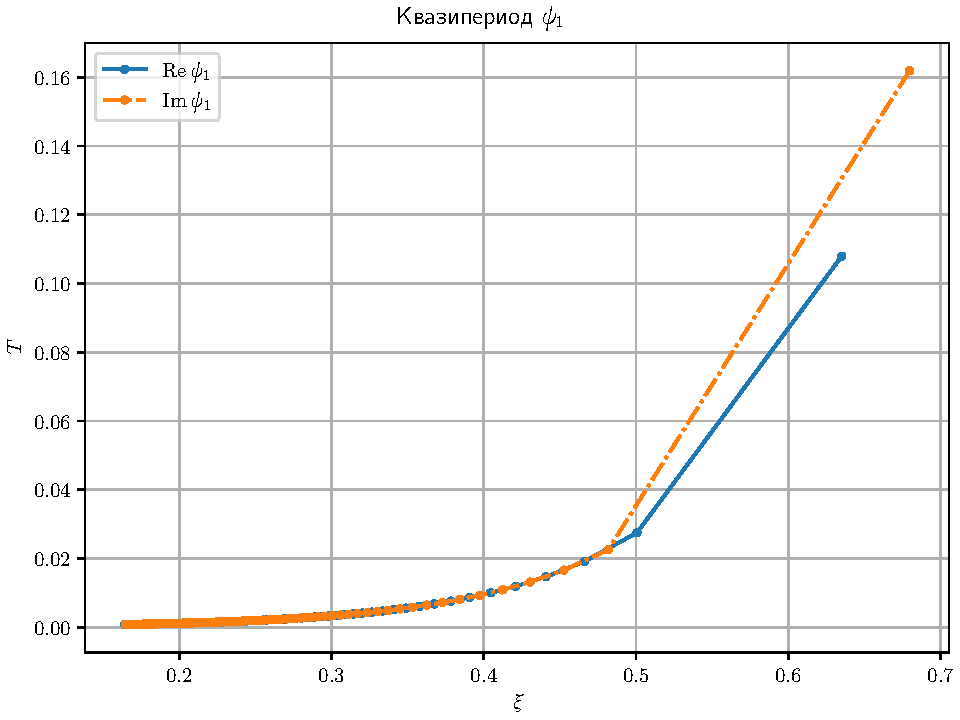
\includegraphics[width=0.8\linewidth]{../data/magexp/figs/RIpsi1_width-ru}
	\caption{\label{fig:magRIpsi1_width}График зависимости длины квазипериода \(\Re\psi_1\) и \(\Im\psi_1\) от \(\xi\) по данным M4}
\end{figure}

Нам стало интересно насколько чаще реальная и мнимая часть \(\psi_{2,3}\) пересекают ось абсцисс по сравнению с реальной и мнимой частью \(\psi_1\) соответственно. Для этого мы посчитали количество занулений реальной и мнимой частей \(\psi_{2,3}\) на интервалах ранее посчитанных квазипериодов реальной и мнимой частей \(\psi_1\) соответственно. Основываясь на этих данных, мы построили графики рис. \ref{fig:magRIpsi2_trans}, \ref{fig:magRIpsi3_trans}. Заметные на графиках выбросы, как мы считаем, являются особенностью работы алгоритма вычисления количество нулей на отрезке.
	\begin{figure}[H]
	\centering%
	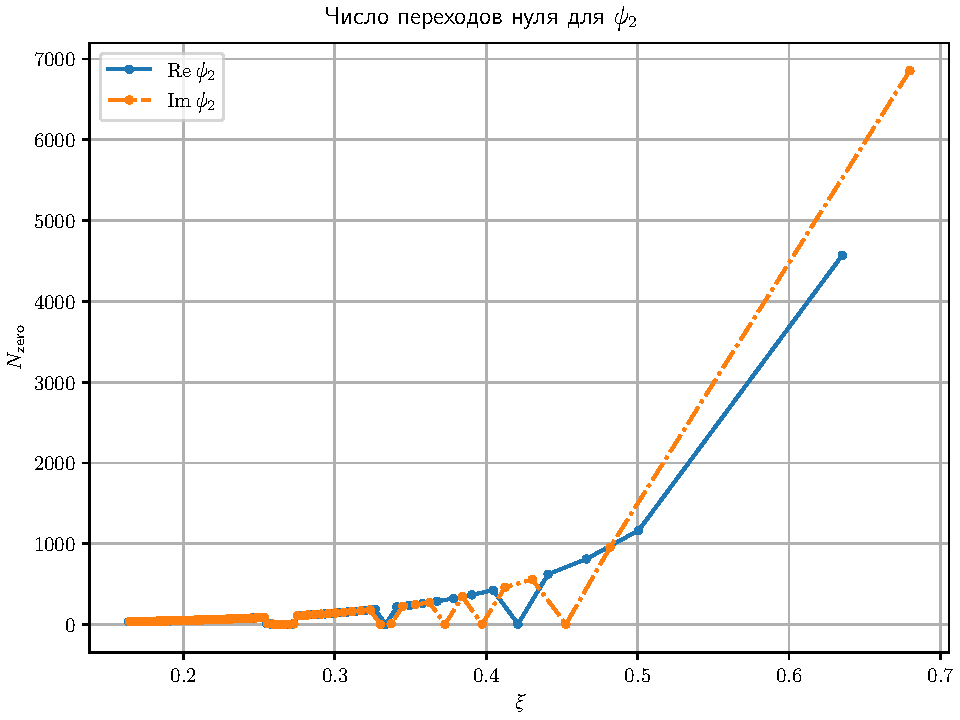
\includegraphics[width=0.8\linewidth]{../data/magexp/figs/RIpsi2_trans-ru}
	\caption{\label{fig:magRIpsi2_trans}График количества переходов через ноль \(\Re\psi_{2}\) и \(\Im\psi_2\) на интервале одного квазипериода \(\psi_1\) по данным M4}
\end{figure}
\begin{figure}[!ht]
	\centering%
	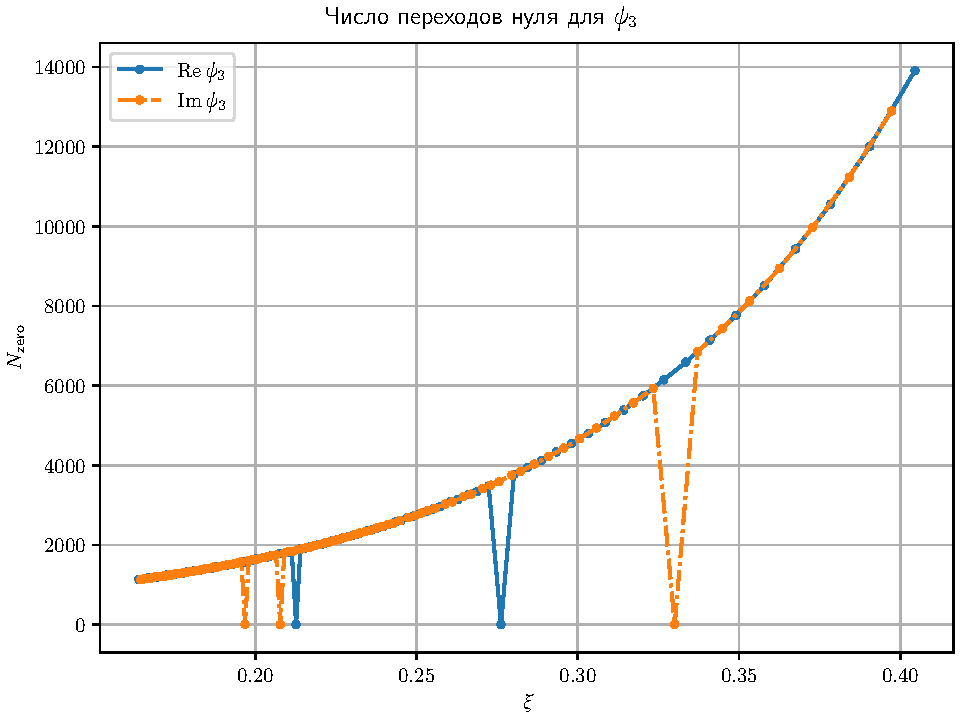
\includegraphics[width=0.8\linewidth]{../data/magexp/figs/RIpsi3_trans-ru}
	\caption{\label{fig:magRIpsi3_trans}График количества переходов через ноль \(\Re\psi_{3}\) и \(\Im\psi_3\) на интервале одного квазипериода \(\psi_1\) по данным M4}
\end{figure}

Обратим внимание, что на графиках для \(\psi_1\)  (рис. \ref{fig:magRIpsi1_width}) мы видим, что величины квазипериодов для реальной и мнимой частей мало отличаются в близких точках. Примерно такое же поведение мы видим в количестве нулей для \(\psi_2\) и \(\psi_3\) (рис. \ref{fig:magRIpsi2_trans}, \ref{fig:magRIpsi3_trans}).

Схожий характер графиков длин квазипериодов \(\psi_1\) и графиков количества переходов \(\psi_{2,3}\) через ноль в квазипериоде \(\psi_1\) позволяет отнормировать данные второй и третьей компоненты по первой. Так, поделив количество нулей \(\psi_{2,3}\) в каждом квазипериоде \(\psi_1\) на длину этого квазипериода. мы получим для каждого квазипериода \(\psi_1\) количество нулей \(\psi_{2,3}\) на единицу длины, или же величину обратную среднему расстоянию между нулями. На рис. \ref{fig:magRIpsi2_rel-trans}, \ref{fig:magRIpsi3_rel-trans} приведены графики основанные на полученных таким образом данных. Их вид очень похож на почти постоянный, если исключить ранее замеченные выбросы. Их почти постоянность можно признать качественным свойством. Их вид подсказывает, что это величина относительно стабильная и может быть использована для качественной характеристики численного решения. Кроме того, для реальной и мнимой частей этот параметр практически один и тот же. Аналогичное поведение мы наблюдаем и для третьей компоненты.

\begin{figure}[H]
	\centering%
	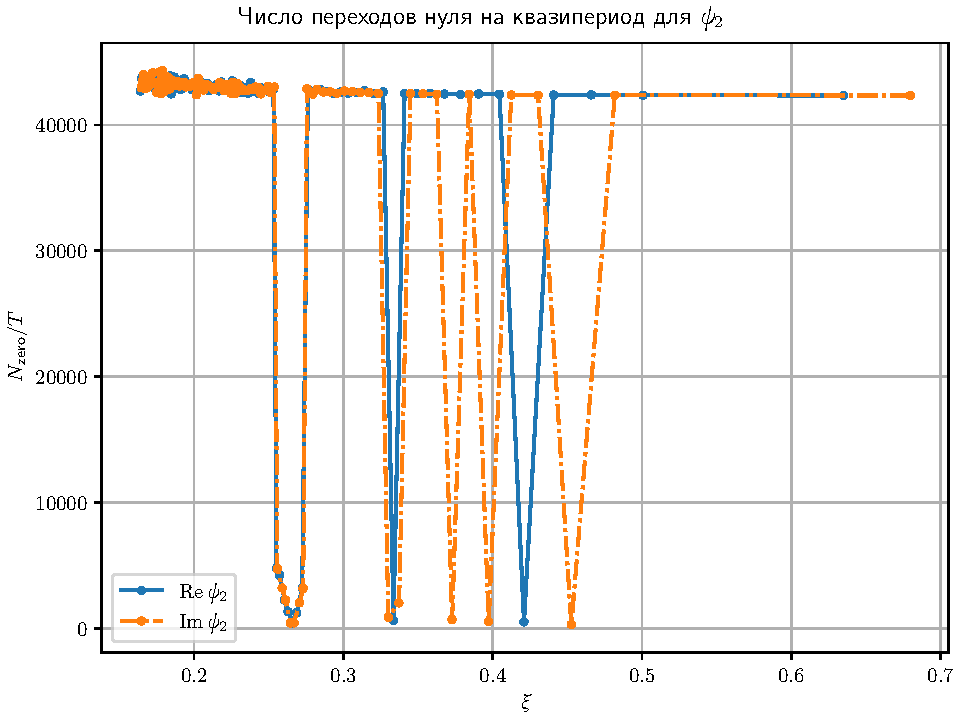
\includegraphics[width=0.8\linewidth]{../data/magexp/figs/RIpsi2_rel-trans-ru}
	\caption{\label{fig:magRIpsi2_rel-trans}График количество нулей \(\Re\psi_{2}\) и \(\Im\psi_2\) на единицу длины квазипериода \(\psi_1\) по данным M4}
\end{figure}
\begin{figure}[H]
	\centering%
	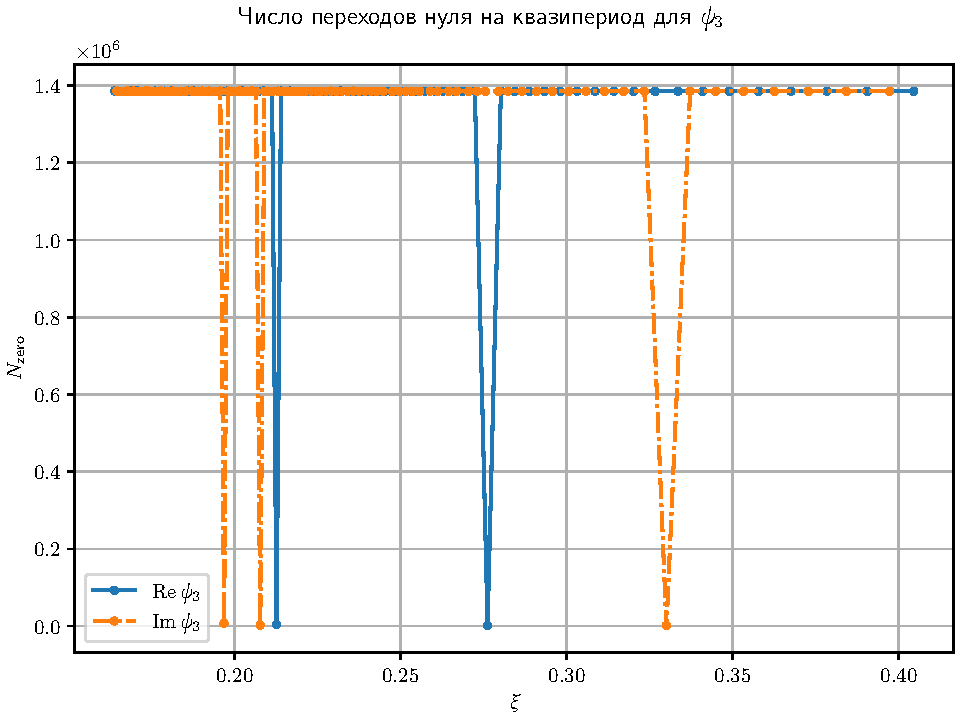
\includegraphics[width=0.8\linewidth]{../data/magexp/figs/RIpsi3_rel-trans-ru}
	\caption{\label{fig:magRIpsi3_rel-trans}График количество нулей \(\Re\psi_{3}\) и \(\Im\psi_3\) на единицу длины квазипериода \(\psi_1\) по данным M4}
\end{figure}

В прил. \ref{app:py} приведен код с помощью которого были получены данные о квазипериодах \(\Re\psi_1\) и \(\Im\psi_1\), а также количестве занулений функций \(\Re\psi_{2, 3}\) и \(\Im\psi_{2, 3}\) в интервалах ранее посчитанных квазипериодов \(\Re\psi_1\) и \(\Im\psi_1\). Усечённые графики, не включающие выбросы приведены в прил. \ref{app:m4_bez}.
	

	\newpage
	\section*{Заключение}
	\addcontentsline{toc}{section}{Заключение}
	В работе рассматривались качественные характеристики численного решения уравнения осцилляций нейтрино в среде \eqref{eq:15}. Применение метода Магнуса позволило выявить, что количество занулений реальной и мнимой части \(\psi_{2,3}\) на единицу длины квазипериода реальной и мнимой части \(\psi_{1}\) является качественной характеристикой численного решения, и она совпадает при использовании разных методов.

	Напоследок отметим, что для уменьшения риска человеческой ошибки были разработаны сценарии для  автоматизации большинства операций.


\newpage
\bibliography{biblio}
\bibliographystyle{ugost2008}
\addcontentsline{toc}{section}{Список литературы}

\newpage
\appendix

\newpage
\section{Графики по данным M4, без выбросов}
График количество нулей \(\Re\psi_{2,3}\) и \(\Im\psi_{2,3}\) на единицу длины квазипериода \(\psi_1\) по данным M4 очень похож на почти постоянный, если исключить выбросы. Но из-за этих самых выбросов масштаб оси \(\dfrac{N_{\text{zero}}}{T}\) большой. Поэтому рассмотрим такие графики не включающие выбросы.

\label{app:m4_bez}
	\begin{sidewaysfigure}
 		\centering%
		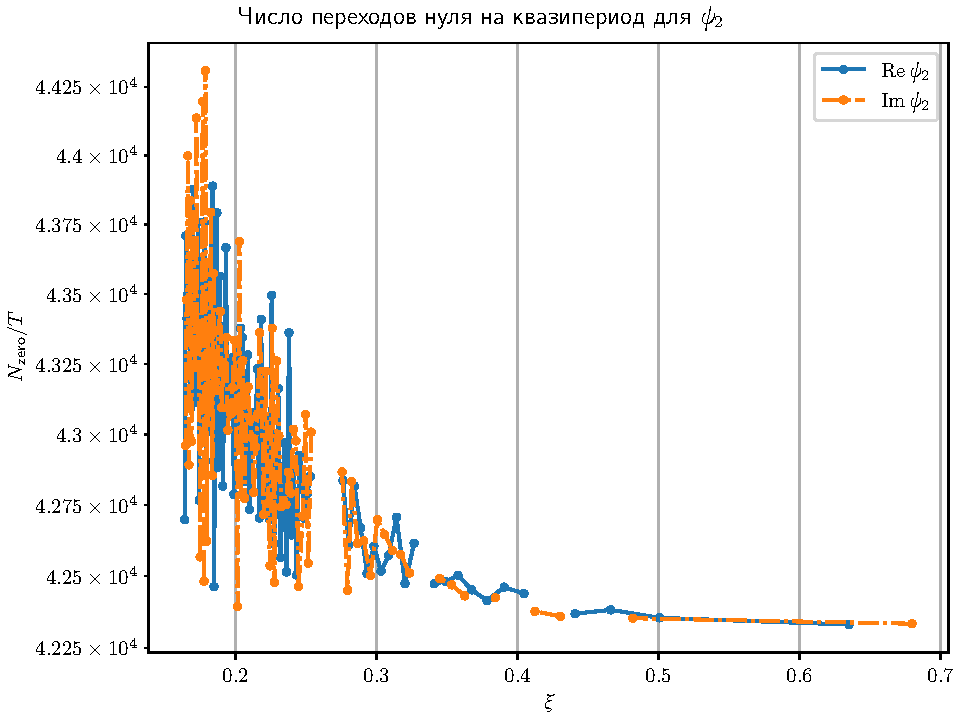
\includegraphics[scale=1.2]{../data/magexp/figs/RIpsi2_logrel-transCUT-ru}
		\caption{\label{fig:magRIpsi2_logre}График количество нулей \(\Re\psi_{2}\) и \(\Im\psi_2\) на единицу длины квазипериода \(\psi_1\) по данным M4, без выбросов}
	\end{sidewaysfigure}
	\begin{sidewaysfigure}
 		\centering%
		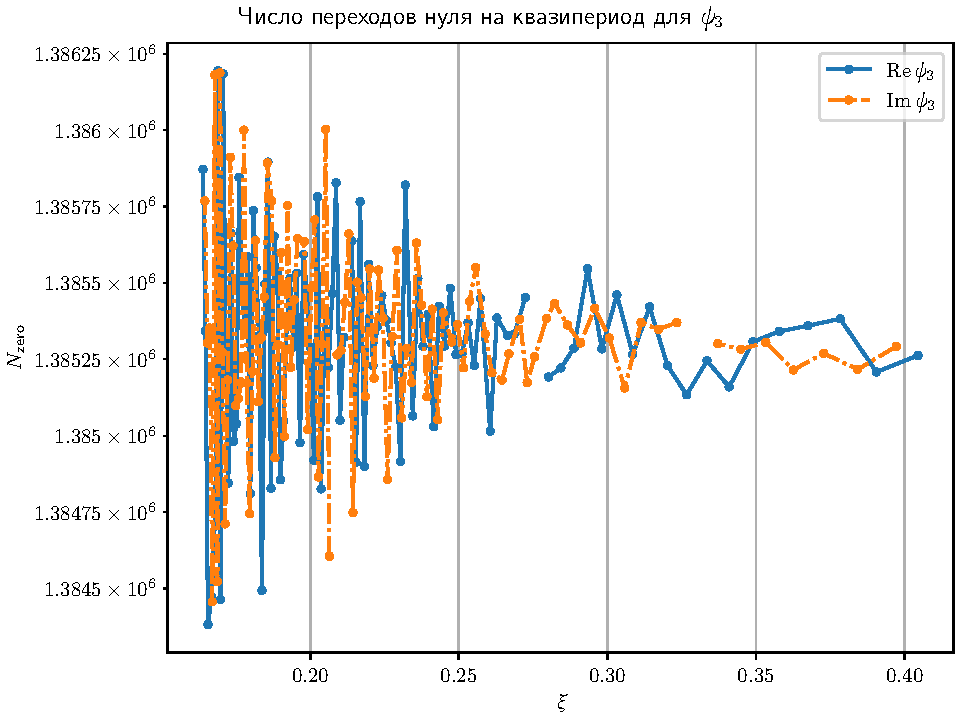
\includegraphics[scale=1.2]{../data/magexp/figs/RIpsi3_logrel-transCUT-ru}
		\caption{\label{fig:magRIpsi3_logre}График количество нулей \(\Re\psi_{3}\) и \(\Im\psi_3\) на единицу длины квазипериода \(\psi_1\) по данным M4, без выбросов}
	\end{sidewaysfigure}

\newpage
\section{Код в Python для решения уравнения осцилляции нейтрино в среде}
\label{app: code-python-vis}

Для численного решения уравнения \eqref{eq:15} использовался код на python. 


Ниже представлен код сценария использованного для получения данных по квазипериодам \(\Re \psi_1(\xi)\), \(\Im\psi_1(\xi)\) в зависимости от \(\xi\), а также данных по количеству переходов через ось абсцисс \(\Re\psi_{2, 3}\) и \(\Im\psi_{2, 3}\) на интервале каждого из ранее найденных квазипериодов \(\Re\psi_1\) и \(\Im\psi_1\) соответственно. 

Его также можно найти в репозитории \url{https://github. com/Fest-Fut/Kursovay}.

\inputminted[linenos,breaklines,fontsize=\scriptsize]{python}{../run.py}

%\textattachfile{stat-prop_v2.py}{Код в виде прикреплённых данных (только для
%	электронной версии документа).}

\label{app:py}

\end{document}

